\section{Parallelization using the CPU}

% -------------------------------------------------------------------------------------- %

\subsection{CPU Architechture}

When referring to CPU architecture one typically either means 
\emph{instruction set architecture (ISA)} when referring to a range of CPUs, or the 
\emph{microarchitechture} of a specific CPU model. The ISA is the blueprint for a set of 
abstract characteristics such as supported instructions, data types, register count, etc. 
The microarchitechture is the \emph{implementation} of this blueprint for a CPU. We 
restrict to the discussion of the microarchitecture for the Intel 3rd gen (Ivy Lake) 
line of processors, though the level of detail is low enough that the statements will 
apply to most modern CPUs built on the x86 64-bit ISA. \\

A processor microarchitecture can be further split to 3 components: 

\begin{itemize}
    \item The front end, which consists of instruction cache and instruction fetch / decode 
    units. This is responsible for fetching batches of instructions from memory, storing 
    the batches in the instruction cache, and decoding the instructions into a set of 
    \emph{micro-operations, or $\mu$Ops}.
    \item The back end (or execution engine), which includes the reorder buffer, 
    unified scheduler (also called reservation station), and various execution ports. 
    Since not all instructions are necessarily dependent on one-another, they often be 
    reordered, or multiple instructions can be executed simultaneously. This is known as 
    \emph{out-of-order execution}. The reorder buffer stores the the \emph{order} of 
    $\mu$Ops until they are retired. The scheduler takes $\mu$Ops and dispatches them to 
    the various ports, each of which is specialized for a subset of instructions. 
    \item The memory system. This includes (typically) three cache levels: L1, L2, and L3.
    The L1 cache is faster than L2, but has a lower storage capacity. The same holds for 
    L2 vs L3 cache.
\end{itemize}

\begin{figure}[ht]
    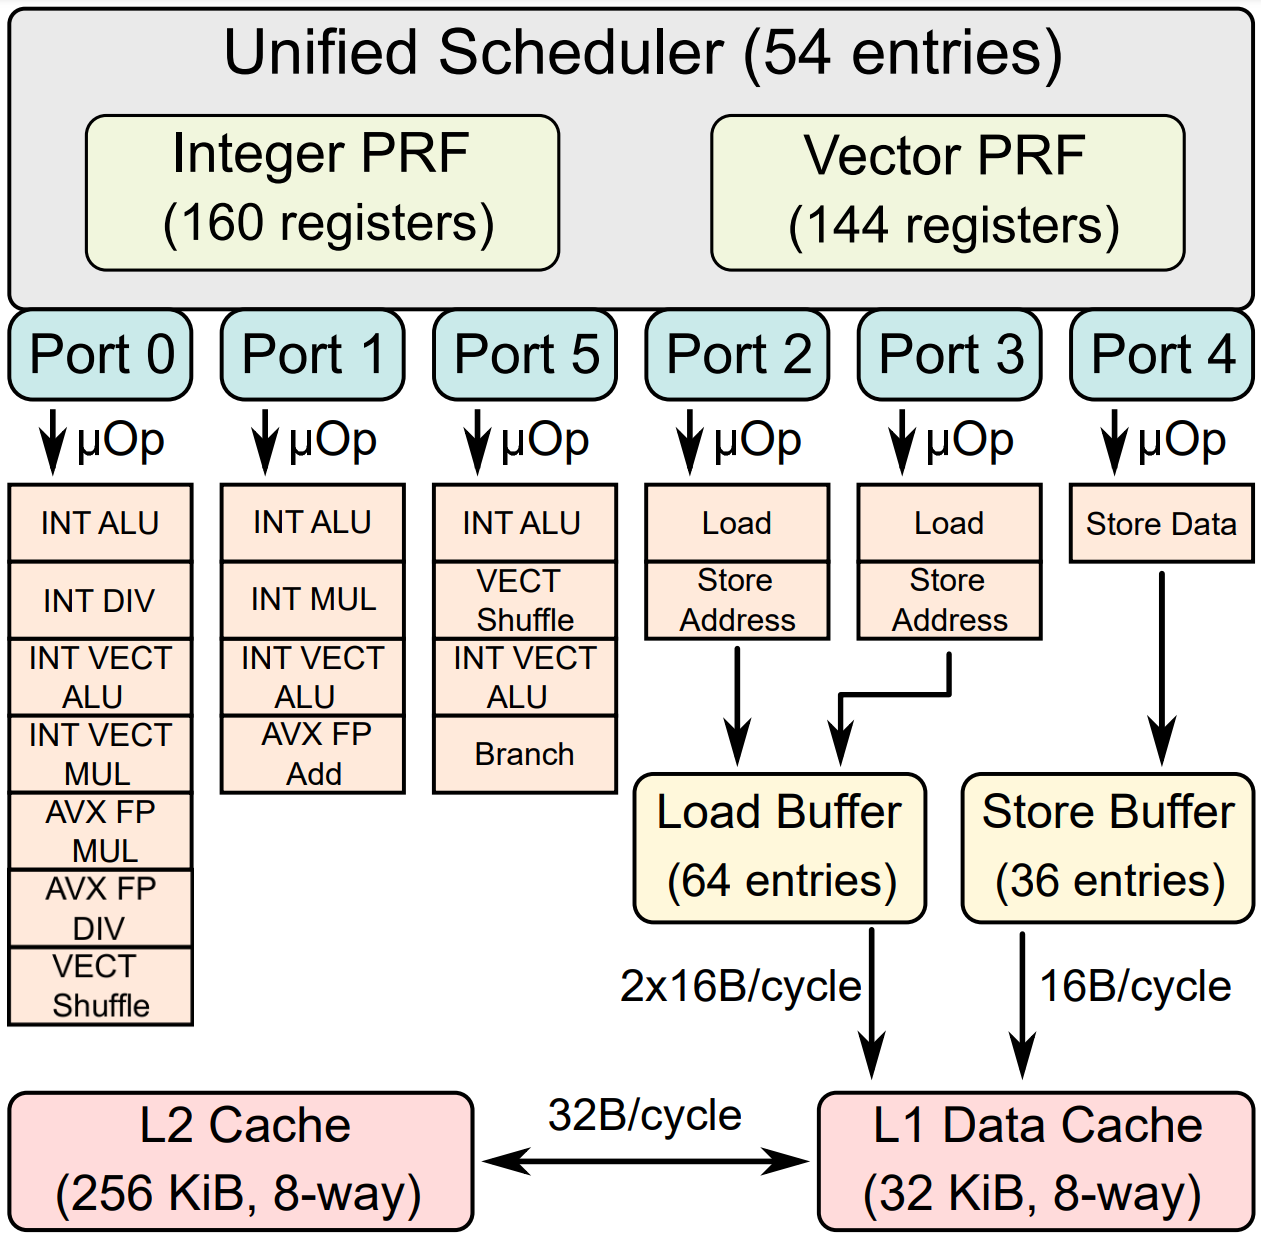
\includegraphics[width=0.6\textwidth]{CPU.png}
    \centering
    \caption{\cite*{solvercomp} Back end for the Intel Ivy Bridge architecture.}
    \label{fig:CPU}
\end{figure}

All three can be limiting factors in a computation, though we will mainly consider 
optimizations for the back end. \\

The simplest technique to increase performance is to utilize the whole instruction set 
available in the acrhitecture. Obviously it can't be expected that the programmer 
optimizes for every microarchitecture and every instruction; if that were true we would 
all be writing pure assembly language. But there are some easy changes one can make, 
primarily using \emph{fused-multiply-add (FMA)} instructions. An example from 
\cite*{solvercomp}: consider the simple dynamical system over $\mathbb{R}$:

\begin{equation}
    x_{k+1} = x_k^2 + p
\end{equation}

for some $p$. To perform one iteration, the CPU needs to call \texttt{MUL} once and then 
\texttt{ADD} once, both of which have latency of roughly 5 clock cycles. Using 
\texttt{FMA}, this can be performed in one operation, nearly doubling performance. A 
consequence of this is that code which does not harness FMA instructions can harness at 
most half of the peak theoretical power of the CPU. \\

In julia, this can be performed with the \jlinl{@muladd} macro from \texttt{MuladdMacro.jl} 
\cite*{muladd}, which automatically converts all combinations of multiply and add into 
calls to the inbuilt \jlinl{muladd} function. \\

Our main technique for parallelization on the CPU is the 
\emph{Advanced Vector eXtension (AVX)}. The philosophy of AVX was initially characterized 
in \cite*{simd} as \emph{Single Instruction Multiple Data (SIMD)}. As the name would 
suggest: when a single instruction, eg. \texttt{ADD}, needs to be applied to multiple 
floating point numbers, then one could pack 4 double precision or 8 single precision 
floating point numbers into a single \emph{vector} stored into the YMM (vector) register. 
Two of these vectors can then be passed into port 1 to the AVX floating point 
arithmetic-logic-unit (AVX FP ADD in \autoref{fig:CPU}), and added all at once. This 
reduces the execution time from 20 clock cycles (4 double precision add operations at 5 
clock cycles each) to just 5 clock cycles (1 packed add operation at 5 clock cycles). \\

The majority of modern compilers can automatically convert simple loops and vectorized 
functions into SIMD instructions. This however is not gauranteed, as the compiler neeeds 
to first prove that there are no data dependencies. Hence to reach peak CPU performance, 
it is often required to manually vectorize. 

% -------------------------------------------------------------------------------------- %

\subsection{Implementation in GAIO.jl}

We wish to map an array of test points 
$x = (x_1,\ x_2,\ \ldots,\ x_n),\,\ x_i \in \mathbb{R}^d$ forward, with as much 
parallelism as possible. For example, consider for $d=3$ and a box $[0,1]^3$ the test 
points:

\begin{jllisting}[language=julia, style=jlcodestyle]
    x = [   # each vector is seen as a point in 3d space
        [1., 0., 0.],
        [0., 1., 0.],
        [0., 0., 1.],
        [0., 0., 0.]
        # etc ...
    ]
\end{jllisting}

We could equivalently characterize this array as an array of packed floats in 
the "packed" space $(\mathbb{R}^4)^3$:

\begin{jllisting}[language=julia, style=jlcodestyle]
    x = [   # three 4xFloat64<...> are seen as a point in our "packed" 3d space
        [
            4xFloat64<1., 0., 0., 0.>, 
            4xFloat64<0., 1., 0., 0.>, 
            4xFloat64<0., 0., 1., 0.>
        ]
        # etc ...
    ]
\end{jllisting}

So our job becomes managing indices careully to convert from one vector of vectors to a 
vector of packed vectors, and vice versa. Hence consider the vector $i$ of indices of $x$:

\begin{equation}
    i = (\ 
        \underbrace{1,\ 2,\ 3,}_{\text{first point}}\quad 
        \underbrace{4,\ 5,\ 6,}_{\text{second point}}\ 
        \ldots,\ 
        \underbrace{3n-2,\ 3n-1,\ 3n}_{\text{nth point}}
    \ )
\end{equation}

% -------------------------------------------------------------------------------------- %
